\documentclass{article}

\usepackage{amsmath}
\usepackage{graphicx}
\usepackage{color}
\usepackage{algorithm}
\usepackage[noend]{algpseudocode}
\usepackage{varwidth}% http://ctan.org/pkg/varwidth
\usepackage{xspace}
\usepackage{placeins}
\usepackage[margin=0.5in]{geometry}
\usepackage{amsfonts}
%\theoremstyle{definition}
%\newtheorem*{dfn}{A Reasonable Definition}


\DeclareMathOperator*{\argmin}{arg\,min}


\title{Derivative Free Model-Based Methods for Local Constrained Optimization}
\author{Trever Hallock}
%\institute{CU Denver}
%\date{January 6, 2012}
% Remove the % from the previous line and change the date if you want a particular date to be displayed; otherwise, today's date is displayed by default.

\makeatletter
\def\BState{\State\hskip-\ALG@thistlm}
\makeatother

\let\oldref\ref
\renewcommand{\ref}[1]{(\oldref{#1})}

\begin{document}


\algnewcommand{\algorithmicgoto}{\textbf{go to}}%
\algnewcommand{\Goto}{\algorithmicgoto\xspace}%
\algnewcommand{\Label}{\State\unskip}


\maketitle


\tableofcontents

\newpage

\section{Introduction}

This paper will discuss research topics for my research in derivative free optimization (DFO).
It begins with an introduction to derivative free optimization supplemented by some of the recent advancements.
It then details several future research directions and one in particular (filter methods) that has been studied.
The focus is on model-based trust region algorithms for local search within constrained derivative free optimization.

\subsection{Introduction to Derivative Free Optimization}
\subsubsection{What it is}

Derivative free optimization refers to mathematical programs in which derivative information is not explicitly available.
Derivatives cannot be calculated directly, and function evaluations are computationally expensive.
%The number of function evaluations can grow when approximating derivatives that are not given explicitly.
One of the primary goals within derivative free optimization is to solve programs while avoiding as many expensive function evaluations as possible.


\subsubsection{Problem formulations}

This proposal aims to develop derivative-free algorithms for solving constrained nonlinear optimization problems of the form
\[ \begin{array}{ccl} \min & f(x) \\
\mbox{subject to} & c_i(x) \le 0 & i \in \mathcal{I} \\
& c_i(x) = 0 & i \in \mathcal{E}
\end{array}
\]
where at least one of the functions $f, c_i, i \in \mathcal{I} \cup \mathcal{E}$ is a black box function, meaning that we have no information about its derivatives.
%\color{red}
%I had another reference to $S(x)$ I now need to delete......
%\color{black}
% I am scared of this change....


%Derivative free methods consider nonlinear, constrained optimization problems of the form
%
%\begin{equation*}
%\begin{aligned}
%& \underset{x}{\text{minimize}} & & f(x, S(x)) \\
%& \text{subject to} & & c_i(x, S(x)) \leq 0, \; \forall i \in \mathcal{I} \\
%& & & c_i(x, S(x)) = 0, \; \forall i \in \mathcal{E}
%\end{aligned}
%\end{equation*}
%which give rise to different classes of derivative-free problems based on properties of
%$S  : \mathbb{R}^n \to \mathbb{R}^m$,
%$f  : \mathbb{R}^{n+m} \to \mathbb{R}$, and
%$c_i: \mathbb{R} \to \mathbb{R}$.
%Here, $S(x)$ is a black-box function, 
%However,  $f$, and $c_i, i \in \mathcal I \cup \mathcal E$ are a priori functions, which can be directly evaluated.
%Although derivatives of $S$ are not known, 
%we will assume that it has nice properties, such as being twice continuously differentiable.
%In other applications, $S$ may be corrupted by noise.

We will introduce several different forms this problem can take noting those which we will discuss algorithms for.
For a more comprehensive characterization of the types constraints, consult \cite{DUMMY:typesofconstraints}.


\subsubsection{Where problems come from}

\color{red}
laziness and parameter tuning were circled.


There are a growing number of applications for DFO. 
For example, derivative free methods can be useful when the objective is the result of a simulation that does not admit automatic differentiation.
As the popularity of complicated simulations increase, so does the demand for optimizing over black box software codes.
 which may be copyrighted.
Derivative free optimization has also been a popular method for parameter tuning, as simulations may have several parameters with unidentified relationships to their output.

\color{black}




Sometimes user laziness can preclude derivative information.
Even when it would be possible to compute derivative information, it may be prohibatively time consuming.

A trend within derivative free optimization is the permission for larger tolerances within solutions.
Their functions are frequently expensive to evaluate, so we can only ask for a small number of significant figures.
This implies slightly less concern for asymptotic convergence rates.

%The general strategy is to converge to a first or second order critical point while evaluating the function as few times as possible.

%\color{blue}
%Your outline mentions iterative methods.
%Should I say something about them?
%I think this is good enough, unless you had more specifics...
%\color{black}

%\underline{\hspace{8cm}}
%
%\color{red}
%An intriguing form of the previous program is presented by \cite{DUMMY:Biegler} and given here:
%\begin{equation*}
%\begin{aligned}
%& \underset{x}{\text{minimize}} & & f(x, y, z) \\
%& \text{subject to} & & g(x, y, z) \leq 0 \\
%& & & h(x, y, z) = 0 \\
%& & & y = S(x) \;  \\
%\end{aligned}
%\end{equation*}
%where
%$S : \mathbb{R}^n \to \mathbb{R}^m$,
%$f : \mathbb{R}^{n+m+k} \to \mathbb{R}$,
%$g : \mathbb{R}^{n+m+k} \to \mathbb{R}^{|\mathcal{I}|}$, and
%$h : \mathbb{R}^{n+m+k} \to \mathbb{R}^{|\mathcal{E}|}$.
%
%Biegler assumes that the dimension of $x$ is small compared to the dimension of $y$ and $z$.
%This permits the algorithmic approach of relaxing $y=S(x)$.
%
%\color{black}
%\underline{\hspace{8cm}}

\subsubsection{Noise. Deterministic versus stochastic}

One branch of DFO is concerned with noisy evaluations of $S$.
Noisy functions can be categorized as either deterministic or stochastic.
Roundoff error, truncation error and finite termination errors can result in what is called deterministic noise.
This means that although a function is not evaluated accurately, the error will not change across multiple function calls with the same input.
On the other hand, stochastic noise means that each point in the domain is associated with a distribution of possible values $S$ may return.
In this paper we assume $S$ is not noisy.

\subsubsection{Types of constraints}

% If $c(x, S(x)) = c(x)$, then 
Sometimes the derivatives of $c$ are known, so the objective is the only derivative free function.
One common such case is to include bound constraints of the form $b_{L} \le x \le b_{U}$ for some $b_{L} < b_{U}$, which gives rise to Box Constrained DFO (BCDFO).
This is one of the better studied cases, with several software packages available, SPBOX, PSwarm, all NLopt algorithms except COBYLA (BOBYQA, NEWUOA, PRAXIS, Sbplx).


We are primarily interested in the case where no derivative information of $c$ is known: for example, if they are also output from a simulation used to evaluate the objective.
This means that each call to the objective gives values of the constraints as well, and vice versa.
% This produces $c(x, S(x))=c(S(x))$.

This means that we have as many points for which we know the constaints as points for which we know the objective.
This creates an interesting situation within model-based approaches which use different orders of models for the objective than the constraints.
The algorithm designer must decide how to choose a subset of these points, use a higher order model, or fit an overdetermined model.

If the constraints can be evaluated at points outside the feasible region, the constraints are called \emph{relaxable} constraints.
Some problems additionally contain ``hidden" constraints which are not explicit in the model but merely result in a notification that the objective could not be evaluated at the requested point.
For example, this can arise when simulation software fails.
This may mean that it is not possible to tell how close to a ``hidden" constraint an iterate lies.


Another area that received attention recently is that of imposing structure on $f$, and $c$.
For example, a method called Practical Optimization Using No Derivatives for sums of Squares
is developed within \cite{DUMMY:leastsquares} when $f$ takes the form of a least squares error
$f(x) = \frac 1 2 \|F(x)\|^2$ over bound constraints where $F$ is a nonlinear, vector valued function.

%Many DFO methods simply let $f(x,S(x)) = S(x)$.



\subsubsection{Importance of Derivatives}

The lack of derivative information means that DFO methods are at a disadvantage when compared to their counterparts in nonlinear optimization.
First and second derivative information is explicit in algorithms with quadratic convergence such as Newton's method.
They are also present in conditions for convergence results such as Wolf's, Armijo or Goldstien for line search methods.
Additionally, stopping criteria usually involve a criticality test involving derivatives.
When derivatives are known, they should be used.
% For this reason, it is desirable for $n$, the dimension of $x$, to be small.


\subsection{Proposed Thesis Direction}

%Within this section, we will discuss the details of what I propose to study.

\subsubsection{Main idea}

The focus of the research will be on developing model-based trust region methods.
Our strategy will be to adapt classical (derivative-based) methods for constrained nonlinear programming to the derivative-free context.
The main idea will be to use function values calculated on a set of sample points to construct local models of the black box functions.
Then, wherever derivatives are required in the classical algorithm, derivatives of the model functions will be used instead.
Of course, other modifications will be needed to achieved desired convergence properties.

In the following section, I give an overview of fundamental concepts of model based methods, particularly trust region methods, along with a review of recent literature.
I will then describe preliminary work on a trust region sequential quadratic programming (SQP) filter method based on \cite{DUMMY:SQPFilter}.
Finally, I describe several ideas for future research.

%Future work includes adapting classical nonlinear optimization algorithms to a derivative free context.
%We start by choosing a nonlinear optimization algorithm, such as the ones listed below.
%The algorithm will contain steps that reference derivatives, for example, in either computation of a step direction or in a criticality measure.
%To convert the algorithm to a DFO context, the derivative evaluations are replaced with derivatives of a model function over a trust region.
%These model functions are constructed from function values at selected sample points.
%, and are trusted to be accurate locally.

%However, once this has been done, the algorithm may require further modifications to ensure convergence.
%For example, in the example we give later of converting the filter method, we had to change trust region management rules to ensure convergence.
%Not only did the trust region simply not go to zero in the filter method which is required in the DFO context, but we needed to decrease the trust region with a weakened criticality measure.
%Other times, small optimizations can be made to avoid unnecessary function calls.

\subsubsection{Potential NLP algorithms to adapt}

There are several considerations to make when selecting an NLP method.
One of the primary concerns is how well it is extended to the trust region framework: 
for example, this conflicts with several goals of line searches as discussed in \ref{linevsmodel}.

Another concern is that some algorithms only produce feasible iterates once the algorithm has converged.
This is different than ``any time algorithms" that maintain feasibility so that the algorithm can be stopped at any time to yield feasible guess.
The longer an any time algorithm is run, the better the returned value is, until optimality is reached.

Here we outline several potential nonlinear programming algorithms of interest.
For some of these algorithms, others have made progress in translating to a DFO context.

\paragraph{Line Search}
Line search is one type of algorithm researchers have made progress in adapting to the derivative free context \cite{DUMMY:FasanoLLR14}.
\paragraph{Filter method}
The first filter methods in DFO were introduced in 2004 within the context of pattern searches \cite{DUMMY:filterpattern}.
Since then, other papers have made progress in a trust region framework including \cite{DUMMY:Biegler} and \cite{DUMMY:Brekelman}.
\paragraph{Active Set}
Active set methods have been considered for DFO \cite{DUMMY:activeset1}, although the focus has been on bound constrained optimization.
\paragraph{Augmented Lagrangian}
A popular method for NLP is the Augmented Lagrangian method, which has also been adapted for both general and box constrained derivative free optimization \cite{augmented}.
\paragraph{Penalty Methods}
Several researchers have considered derivative free algorithms for penalty methods including \cite{DUMMY:LiuzziLS10}.
There are many flavors of these algorithms.

\paragraph{Interior Point}
% I used to have a reference for this one.

%\item Progressive Barrier


% I have not been able to find the paper that listed such a nice compact list of references to different algorithms in a derivative free context.
% It might be on my hard drive for my school desktop.

%\begin{itemize}
%	\item Penalty
%	\begin{itemize}
%		\item Abramson \& Audet, 2006
%		\item Abramson et al. 2009c
%		\item audet et al. 2008b
%		\item Audet \& Dennis, 2006
%		\item sequential penalty merit functions Liuzzi et al., 2010
%		\item smoothed exact $l-\infty$ penalty function Liuzzi \& Lucidi, 2009
%		\item exact penalty merit function Fasano, Liuzzi, Lucidi, \& Rinalsdi, 2014; Gratton \& Vicente, 2014
%	\end{itemize}
%	\item Progressive Barrier
%	\begin{itemize}
%		\item Audet \& Dennis, 2009
%	\end{itemize}
%\end{itemize}

%\subsubsection{Overview of the rest of the paper}
%
%In the remaining pages, we will discuss DFO background by discussing high level characterizations of DFO methods and some of the issues these methods face.
%We will finish the background with a brief literature review before discussing one classical NLP algorithm I converted to a derivative free context.
%Finally, we will briefly mention some of the interesting specializations that can be pursued.

\section{Background}
\subsection{Derivative Free Algorithm classes}
\subsubsection{Automatic Differentiation}

When $S$ is the result of a simulation for which the source code is available, one convenient approach is to perform automatic differentiation.
Although derivatives of complicated expressions resulting from code structure are difficult to work with on paper, the rules of differentiation can be applied algorithmically.
However, the nature of the code or problem can make this very difficult: for example with combinatorial problems that rely heavily on if statements.

\subsubsection{Direct search}


Another approach is to use direct search methods that do not explicitly estimate derivative information but evaluate the objective on a pattern or other structure to find a descent direction.
Examples of this include Coordinate descent, implicit filtering and other pattern based search methods.
One of the most popular direct search method is Nelder Mead, which is implemented in fminsearch in Matlab.
It remains popular although it is proven to not converge in pathological cases unless modifications are made.

These methods can be robust in that they are insensitive to scaling and often converge to a local minimum even when assumptions such as smoothness or continuity are violated.
However, they ignore potentially helpful information because they do not use derivative information provided through the function evaluations.
This means that they can also lack fast convergence rates.

%\color{red}
%(0th derivative)
%\color{black}

\subsubsection{Finite difference methods}

Finite difference methods can be used to approximate the derivative of a function $f$.
One common approximation called the symmetric difference is given by $\nabla f(x) \approx (\frac{f(x+he_i) - f(x-he_i)}{2h})_i$ for some small $h$ where $e_i = (0,\ldots, 0, 1, 0, \ldots, 0)^T \quad \forall \; 1 \le i \le n$ is the unit vector with $1$ in its $i$th component.
%This may work well, but can have issues with unlucky iterates (CITE).
However, the number of function evaluations tends to grow large with the dimension and number of iterations the algorithm performs.
This is because derivative information is only gathered near the current iterate when $h$ is small, which is required for accurate derivative calculations.
Because of the large number of function evaluations required for finite difference schemes, it may preferable to spread sample points out over the entire region where we may expect to step.
Also, function evaluations may be subject to noise, making the finite difference approximations of derivative problematic.

\subsubsection{Model based methods}

In this paper, we are concerned with model based methods.
These typically minimize a model function that only approximates the objective and constraints.
The model functions are chosen to accurately represent the original function, but allow for derivative information to be calculated easily.
They work by evaluating functions on a set of sample points to construct local models of the functions.

This allows the algorithm to minimize these easier model functions over a trust region, rather than working with the original function.
When derivatives are given in the original function, model-based methods can also be used to approximate derivative information.
We will see several examples in what follows.


%\color{red}
%Kriging seems to be another popular model function, but I usually see it used within global optimization.
%\color{black}




\paragraph{Interpolation/regression methods}

Within Interpolation methods, we construct our model by regressing basis functions onto a set of sampled points.
For example, given a function $f(x) : \mathbb R^n \to \mathbb R$ we can use a set of basis functions $\phi_i : \mathbb R^n \to \mathbb R \quad \forall 1 \le i \le d_1$ to construct a model function $m(x) = \sum_{i=1}^{d_1} \lambda_i \phi_i(x)$ approximating $f(x)$ by selecting appropriate $\lambda_i \in \mathbb R$.
This is done by choosing a set of sample points
$Y = \{y^1, y^2, \ldots, y^{d_2}\}$,
evaluating $f = (f_1 = f(y^1), f_2 = f(y^2), \ldots, f_d = f(y^{d_2}))^T$ and forcing model agreement with the original function $f(x)$ by ensuring

\begin{equation}
\label{reg}
\begin{bmatrix}
    \phi_1(y^1)      & \phi_2(y^1)       & \ldots & \phi_{d_1}(y^1)      \\
    \phi_1(y^2)      & \phi_2(y^2)       & \dots  & \phi_{d_1}(y^2)      \\
                     &                   & \vdots &                      \\
    \phi_1(y^{d_2})  & \phi_2(y^{d_2})   & \ldots & \phi_{d_1}(y^{d_2})
\end{bmatrix}
\begin{bmatrix}
    \lambda_1      \\
    \lambda_2      \\
    \vdots         \\            
    \lambda_{d_1}
\end{bmatrix}
\approx
\begin{bmatrix}
    f_1      \\
    f_2      \\
    \vdots         \\            
    f_{d_2}
\end{bmatrix}.
\end{equation}

When $d_1 = d_2$ this is called interpolation and equality is desired within \ref{reg}.
When $d_1 < d_2$ this is called underdetermined interpolation.
This can be handled by requesting and a minimum norm solution.
Finally, when $d_1 > d_2$ this is called regression and only a least squares solution can be requested.
Note that in practice, the set $Y$ is shifted and scaled.

\paragraph{Basis functions}

The choice of model functions $\phi_i$ can have some affect on the convergence rate, as Powell showed in \cite{DUMMY:PowellRadialBasis}.
One common choice of basis functions is the Lagrange polynomials, in which we select polynomials satisfying $\phi_{i}(y^j) = \delta_{ij}$, the kroneker delta function.
This reduces the matrix within \ref{reg} to an identity matrix.
Lagrange polynomials of order $p$ can be computed by starting with the monomial basis $\prod_{i=1}^{n} x_i^{n_i}$ for all choices of $0 \le n_i \le p$ with $\sum_{i=1}^n n_i \le p$ and inverting the corresponding Vandermonde matrix.

Newton's Fundamental polynomials are also used, and follow a similar pattern.
However, they maintain different orders of polynomials within the basis:
a single constant value, a set of $n+1$ linear polynomials,
$n + {n \choose 2}$ quadratic functions, and more for higher order polynomials.
Radial basis functions may have some intuitive advantage because the algorithm makes claims about the accuracy of the function over a trust region.


Model functions are usually chosen to be fully linear or fully quadratic: terms describing how the model's error grows as a function of the trust region radius.

\paragraph{Sampling issues}

These methods have issues with poor sampling choices.
The two most important aspects of the sample points are their geometry and proximity.

\subparagraph{Geometry}

For geometry, regression based methods require that the set the function is evaluated at must be $\Lambda$-poised for a fixed constant $\Lambda$.
If the set is $\Lambda$-poised for a certain trust region radius, then the maximum absolute value of any Lagrange polynomial over the trust region is one.
This ensures that the Vandermonde matrix used to find the coefficients used to express the model function in terms of a basis of Lagrange polynomials is well conditioned.
Although we do not go into the details here, problems become apparent when comparing the Lagrange polynomials associated with a poised set with those of an ill poised set.

Within the first set of pictures below we see the set of quadratic Lagrange polynomials on the interval $[-1,1]$.
The maximum value of these polynomials over the trust region is simply $1$.
However, if we use sample points $\{-1, .9, 1\}$ instead of the points $\{-1, 0, 1\}$,
we find the second set of polynomials.

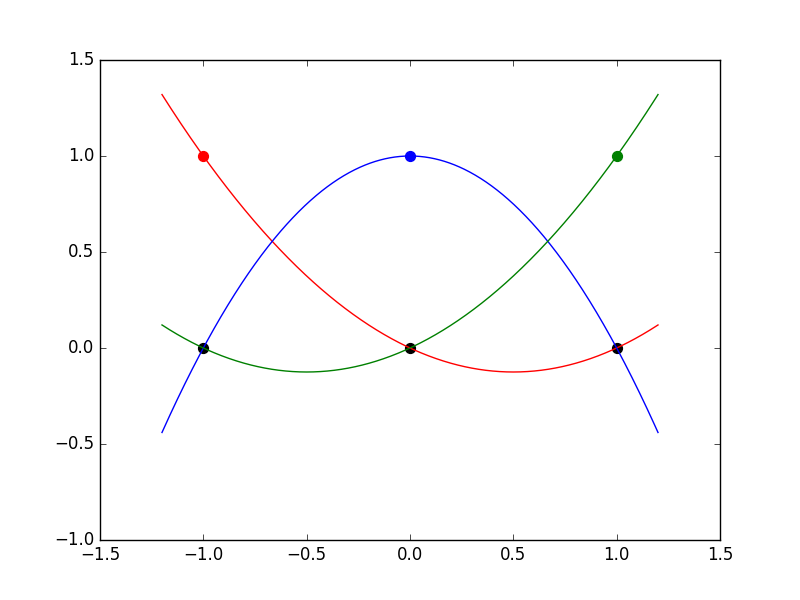
\includegraphics[width=200px]{poised.png}
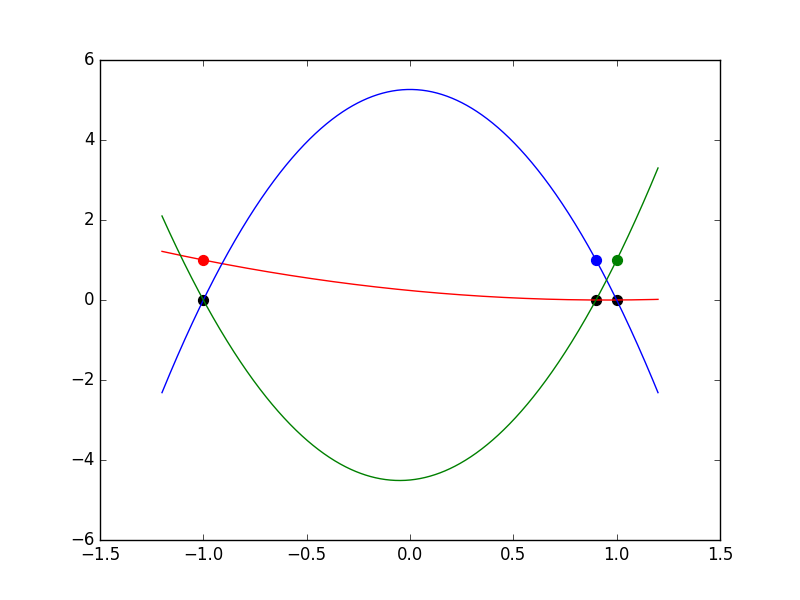
\includegraphics[width=200px]{illpoised.png}

If we use these to approximate $3 + \tan^{-1}(x)$, the first basis functions do not vary far from the objective value over the trust region, and the maximum difference between the function and the model function is $0.0711$.
However, the second basis functions jump far away from the actual function, and the maximum difference between the model function and actual function is 
$0.1817$.

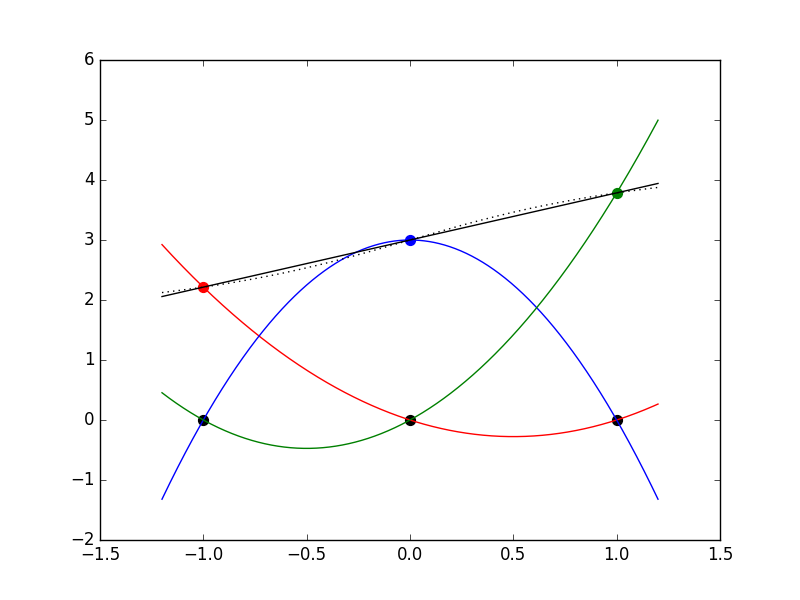
\includegraphics[width=200px]{poised_approx.png}
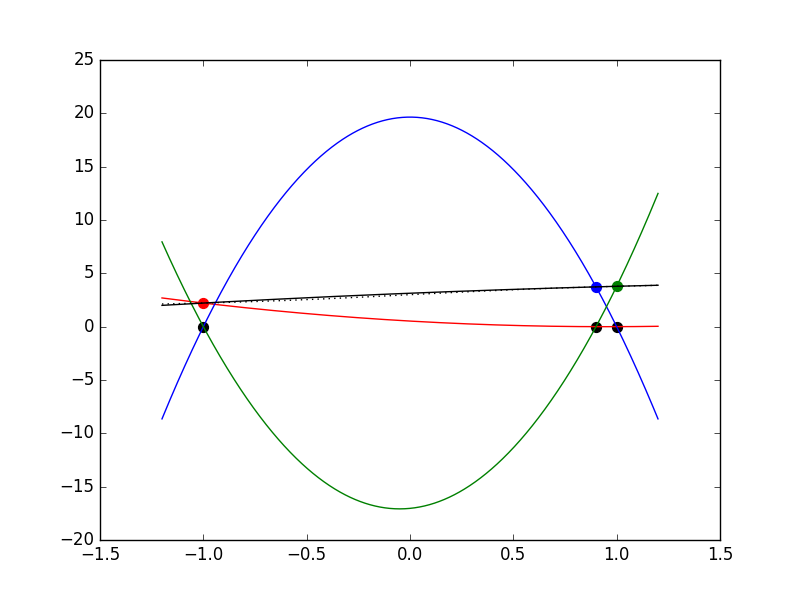
\includegraphics[width=200px]{illpoised_approx.png}

\subparagraph{Proximity}

Proximity refers to the trust region radius.
The trust region must go to zero if we are to be sure that we have reached a critical point.
In general, the smaller the trust region, the closer to linear or quadratic the original function will look.
This is because the model's error term given by Taylor's expansion is proportional to the trust region radius.

%\color{red} Within noisy optimization, this gives rise to several more problems. If you think there is something else about proximity that I should mention, please let me know. \color{black}

\subsubsection{Model-based, Trust Region Methods}

The overall description of the trust region framework is that a set of poised points are chosen for some radius $\Delta>0$ about the current iterate.
The objective and constraints are then evaluated at these points to construct a model function as a linear combination of some set of basis functions.
Next, the model is minimized over this trust region and the argument minimum becomes the trial point.
The objective is evaluated at the trial point and a measure of reduction $\rho$ is computed.
If $\rho$ implies that sufficient reduction has been made and that the model approximates the function well, the trial point is accepted as the new iterate.
Otherwise, the trust region is reduced to increase model accuracy.


For unconstrained optimization, the algorithmic framework can be described with these steps:

\begin{enumerate}
	\item Create a model function $m_k(x)$.
	\begin {itemize}
		\item In classical trust region methods, the following quadratic model function is used:
		\[
		m_k(x) = f(x^{(k)}) + \nabla f(x^{(k)})^T (x-x^{(k)}) + \frac 1 2 (x-x^{(k)})^T\nabla^2f(x^{(k)})(x-x^{(k)})
		\]
	\end{itemize}
	\begin{itemize}
		\item $\nabla f(x^{(k)})$ and $\nabla^2 f(x^{(k)})$ must be approximated
		\item Geometric properties of the sample set that must be satisfied
	\end{itemize}
	
	\item If $\nabla m_k(x) < \tau$ stop, where $\tau$ is some tolerance
	
	\item Solve the Trust region subproblem: $s^{(k)} = \argmin_{s\in B_{x^{(k)}}( \Delta_k)} m_k(x^{(k)} + s)$
	\begin {itemize}
		\item $B_{x^{(k)}}(\Delta_k) = \{ x \in \mathbb{R}^n : \| x - x^{(k)} \le \Delta_k \}$ 
		is the ball of radius $\Delta_k$ centered at $x^{(k)}$
	\end{itemize}
	
	\item Test for improvement
	\begin{itemize}
		\item Compute
\begin{equation}
\label{rho}
\rho_k = \frac{f(x^{(k)}) - f(x^{(k)}+s^{(k)})}{m_k(x^{(k)}) - m_k(x^{(k)}+s^{(k)})}
\end{equation}
which measures the actual improvement over predicted improvement
		\item If $\rho$ is small, $x^{(k+1)}=x^{(k)}$ (reject) and decrease radius
		\item If $\rho$ is intermediate, $x^{(k+1)}=x^{(k)}+s^{(k)}$ (accept) and decrease radius
		\item If $\rho$ is large, $x^{(k+1)}=x^{(k)}+s^{(k)}$ (accept) and either increase the radius or decrease if $\nabla m_k(x_k)$ is small
	\end{itemize}
	
	\item Go to step 1
\end{enumerate}

Our goal is generalize this framework to handle constraints, where we must reduce constraint violation while ensuring the accuracy of the models of the constraints.


\subsubsection{Trust region versus Linesearch} \label{linevsmodel}

Within derivative free optimization, we can ensure the accuracy of our model function by sampling points over a small enough trust region.
However, reducing the trust region implies more points must be evaluated.
Linesearch methods rely on the the ability to calculate a descent direction that will be accurate in a small enough region around the current iterate:
small enough that the trust region must be reduced to ensure the model's accuracy.

This means trust region framework fits into derivative free optimization more naturally than line search methods.
Not only do the trust regions arise naturally, but many line search algorithms exploit how much easier it is to find a descent direction than solve a trust region subproblem.
However, in derivative free optimization, solving a costly trust region subproblem is acceptable if it allows us to avoid even more expensive function evaluations.


% We began with a line search filter method, however we found that this had several drawbacks:
% \begin{itemize}
% \item Line search algorithms exploit how much easier finding a descent direction is than solving the trust region subproblem, but this saved computation is not as useful in DFO as here it is function evaluations that we avoid
% \item As the algorithm backtracks on the step length, the trust region must be reduced, as the models are accurate over a region rather than at a single point
% \end{itemize}



\subsubsection{Literature Background}

\paragraph{Derivative free methods}

Within  \cite{DUMMY:intro_book} derivative-free methods are developed in detail.
This is the first text book devoted to derivative free optimization.
It contains a good explanation of ensuring geometry of the current set with poisedness for unconstrained problems and also covers other derivative-free methods including direct-search and line search.

A good review of derivative free algorithms and software libraries can be found in \cite{DUMMY:review}.
This compares several software libraries, and reviews the development of derivative free optimization since it started.
Another recent review can be found in \cite{DUMMY:review2}.

Within \cite{DUMMY:linesearch_global} and \cite{DUMMY:linesearch_local} Biegler uses a filter method to ensure global convergence within a line search framework.


\paragraph{Filter methods}

The original filter method was proposed by Gould and Toint in \cite{DUMMY:original_filter}.
The motivation for the filter method was that the algorithm does not need to tune any parameters as in penalty or merit methods.
We will discuss filter methods in more detail below.

%A recent paper from September 2016 \cite{DUMMY:Biegler} implements a derivative-free trust region filter method for solving the the program given above (REFERENCE).
%This is more convenient for some problems than the algorithm we consider as it allows for the objective to depend on other glass box functions of the input and multiple outputs of the black box function.
%The authors compare their algorithm to finite difference methods as well as kriging on three different applications from Chemistry. Within the algorithm, the current iterate is always feasible with respect to all inequalities except for the constraint $y=d(z)$.

In the 2006 paper \cite{DUMMY:Fletcher}, Fletcher reviews how filter methods have developed.
The only references to derivative-free versions of the filter method are those applied to pattern based (direct) methods.
However, the authors outline trust region filter methods along with several other variants.

%In Brekelman's paper \cite{DUMMY:Brekelman}, a trust region filter method is developed to minimize function evaluations by constructing linear model functions.
%This paper also uses experimental designs to choose following iterates.

Within \cite{DUMMY:sqp_filter} a sequential quadratic programming method is applied to the filter method?

%Within \cite{DUMMY:linesearch_global} and \cite{DUMMY:linesearch_local} Biegler uses a filter method to ensure global convergence within a line search framework.
%We experimented with this before deciding combining line search with the derivative-free trust region approach was not a natural approach. (There have been attempts to employ both of these frameworks in \cite{DUMMY:CombineTrustAndLine}.)

I based my algorithm on the trust region filter method described in \cite{DUMMY:SQPFilter}.

%Within  \cite{DUMMY:intro_book} derivative-free methods are developed in detail.
%This contains a good explanation of ensuring geometry of the current set with poisedness for unconstrained problems and also covers other derivative-free methods including direct-search and line search.

\paragraph{Derivative free filter methods}

In Brekelman's paper \cite{DUMMY:Brekelman}, a trust region filter method is developed to minimize function evaluations by constructing linear model functions.
This algorithm evaluates the underlying functions at points chosen by an experimental design, 
and moves the design towards otpimality according the filter while making any necessary geometry improvement steps.

%Within \cite{DUMMY:sqp_filter} a sequential quadratic programming method is applied to the filter method?

A recent paper from September 2016 \cite{DUMMY:Biegler} implements a derivative-free trust region filter method for solving the following intriguing program:

\begin{equation*}
\begin{aligned}
& \underset{x}{\text{minimize}} & & f(x, y, z) \\
& \text{subject to} & & g(x, y, z) \leq 0 \\
& & & h(x, y, z) = 0 \\
& & & y = S(x) \;  \\
\end{aligned}
\end{equation*}
where
$S : \mathbb{R}^n \to \mathbb{R}^m$ is a black box function,
$f : \mathbb{R}^{n+m+k} \to \mathbb{R}$,
$g : \mathbb{R}^{n+m+k} \to \mathbb{R}^{|\mathcal{I}|}$, and
$h : \mathbb{R}^{n+m+k} \to \mathbb{R}^{|\mathcal{E}|}$.

Biegler assumes that the dimension of $x$ is small compared to the dimension of $y$ and $z$.
This permits the algorithmic approach of relaxing $y=S(x)$.

This is more convenient for some problems than the algorithm we consider as it allows for the objective to depend on other glass box functions of the input and multiple outputs of the black box function.
Glass box functions, as opposed to black box, are functions for which derivative information is known.
The authors compare their algorithm to finite difference methods as well as kriging on three different applications from Chemistry. 
Within the algorithm, the current iterate is always feasible with respect to all inequalities except for the constraint $y=d(z)$.

Colson has also applied filter techniques to derivative-free optimization in his 2004 Ph.D. thesis \cite{DUMMY:Colson2004}.
This focuses on bilevel programming.

\paragraph{Beyond the filter}
Within nonlinear programming, some new techniques have been proposed extending the filter method.
One new algorithm Toint proposes in \cite{DUMMY:trust_funnel_dfo} generalizes the filter method with the notion of a trust funnel.
This is an interior point algorithm that is suitable for large scale problems, as it is matrix free.
This could be generalized as it is only for glass box functions with no derivative-free methods.



%\color{red}
%We experimented with this before deciding combining line search with the derivative-free trust region approach was not a natural approach. 
%(There have been attempts to employ both of these frameworks in \cite{DUMMY:CombineTrustAndLine}.)
%\color{black}


% In order to give this talk as is, I need to be prepared to talk about
% and preferably have optional slides for
% Coordinate descent, Nelder mead (not implicit filtering http://www4.ncsu.edu/~ctk/imfil.pdf)
% Wolf, Armijo, or Goldstein
% trust region subproblem
% know values of \eta_1, \eta_2
% interpolation may involve frebenius norm/enforcing sparsity
% http://www.sciencedirect.com/science/article/pii/S0167819103000139
% Should use the word black box early on

% the two additional review papers.


%\color{red}
%
%\begin{center}
%\begin{tabular}{ | c | c | c | }
%\hline
% Classical NLP Algorithm & Model based approach & Pattern Search \\ 
%\hline
% SQP Filter & Yes & Maybe \\  
% Trust Funnel & Maybe & Maybe \\
% Penalty Methods & Maybe & Maybe \\
% Barrier Methods & Maybe & Maybe \\
% Augmented Lagrangian & Maybe & Maybe \\
% Interior Point Algorithms & Maybe & Maybe \\
% Filter Methods & Maybe & Maybe \\
%\hline
%\end{tabular}
%\end{center}
%
%\color{black}

\section{Progress}

In this section we discuss one algorithm that has been converted to a derivative free context.
This is the filter method, which has been independently adapted for derivative free optimization by \cite{DUMMY:Brekelman}.
%\color{red}
%(delete this: We first describe the classical algorithm before introducing the changes required for derivative free optimization.)
%\color{black}


\subsection{SQP Filter method}

We will be considering problems of the form


\begin{center}
\begin{align}
\label{problem}
\min_x & \quad f(x) \\
  c_i(x) \le 0   & \quad \forall i \in \mathcal {I} \nonumber \\
  c_i(x)  = 0    & \quad \forall i \in \mathcal {E} \nonumber
\end{align}
\end{center}
where $f : \mathbb R^n \to \mathbb R$, and each $c_i : \mathbb{R} \to \mathbb{R}$.
It will be convenient to write
$c_{\mathcal {I}}(x) = (c_1(x), c_2(x), \ldots, c_{|\mathcal{I}|})^T$,
$c_{\mathcal {E}}(x) = (c_{|\mathcal{I}|+1}(x), c_{|\mathcal{I}|+2}(x), \ldots, c_{|\mathcal{I}| + |\mathcal{E}|})^T$ and
$c(x) = (c_{\mathcal{I}}^T(x), c_{\mathcal{E}}^T(x))^T$.


We work within a trust region, sequential quadratic programming framework with interpolating model functions that uses a filter method introduced by Gould and Toint \cite{original_filter}.
For our algorithm, we assume that all functions are derivative-free: all functions are evaluated by a single call to a black box function:
$S(x) = (f(x), c_{\mathcal {I}}(x)^T, c_{\mathcal {E}}(x)^T)^T$.

We first compute an interpolation set poised for regressing a set of model functions, which we choose to be quadratic functions.
Although we have enough sample points to construct a quadratic model of the constraints, we only construct linear models to avoid the complexity of Quadratically Constrained Quadratic Programming which is NP-hard.

\subsubsection{Model functions}

At an iteration $k$, we first construct a model function $m_f^k(x)$ that we use to approximate the first and second derivatives of $f(x)$.
We also construct $m_{\mathcal{I}}^k(x)$ and $m_{\mathcal{E}}^k(x)$ to approximate the first derivatives of $c(x)$.
Namely, at an iterate $x^k$, we let $f^k = f(x^k)$, $g^k = \nabla m_f^k(x^k)$. %be the gradient of the objective's model at $x^k$.
We also define the $c_{{\mathcal{I}}}^k = c^k_{\mathcal{I}}(x^k)$, 
$A_{{\mathcal{I}}}^k = \nabla m_{\mathcal{I}}^k(x^k)$,
$c_{{\mathcal{E}}}^k = c_{\mathcal{E}}(x^k)$, and
$A_{{\mathcal{E}}}^k = \nabla m_{\mathcal{E}}^k(x^k)$.

We will also need to compute the Hessian of the Lagrangian for \ref{problem}.
The Lagrangian is defined as 
 $L(x, \mu, \lambda) =
 f(x)  
 + \sum_{i \in {\mathcal{I}}} \mu_i     c_i(x)
 + \sum_{i \in {\mathcal{E}}} \lambda_i c_i(x)$.
To compute its second derivative, we let $A^k$ and $c^k$ contain $A_{\mathcal{E}}^k$ and $c_{\mathcal{E}}^k$ as well as any rows of $A_{{\mathcal{I}}}^k$ and $c_{\mathcal{E}}^k$ corresponding
to active constraints at $x^k$.
The set of active constraints $\mathcal A \subseteq \mathcal I \cup \mathcal E$ includes $\mathcal E$ and any $i \in \mathcal I$ for which $c_i(x^k) \ge 0$.
We then solve the system
\begin{align*}
\nabla^2m_k(x_k) & d + {A^k}^T\lambda & = g^k \\
A^k              & d                & = c^k
\end{align*}
for $\lambda$ and compute
\[
H^k = \nabla^2 m_k(x^k) 
+ \sum_{i \in \mathcal E} \lambda_i \nabla^2 m_{g,i}^k(x^k) 
+ \sum_{i \in \mathcal A \backslash \mathcal E} \lambda_i \nabla^2 m_{h,i}^k(x^k).
\]

With these definitions, we define the quadratic subproblem as

\begin{align*}
\argmin_s  f(x^k+s) = f^k + (g^k)^Ts + \frac 1 2 (s^k)^T H^ks^k  &\\
     c_{{\mathcal{I}}}^k + A_{{\mathcal{I}}}^ks       &\le \; 0  \\
s.t. \hspace{1cm} c_{{\mathcal{E}}}^k + A_{{\mathcal{E}}}^ks           &=\; 0 \\
     \| s \|                      &\le \; \Delta_k.
\end{align*}



\subsubsection{Step decomposition}
In each iteration, we attempt to compute a step $s^k$ that will decrease either the constraint violation or the function value. 
To this end, we decompose the step $s^k$ into a normal step $n^k$ intended to decrease constraint violation and a tangential step $t_k$ intended to reduce the objective.
The step $n^k$ projects the current iterate onto the feasible region.
Currently, we project $x^k$ onto only the linear model of the feasible region.
This gives rise to the following definition:

\begin{align}
\label{normal}
 n_k = \argmin_n            \|n\|^2    &\\
     c_{{\mathcal{I}}}^k + A_{{\mathcal{I}}}^kn       &\le \; 0  \nonumber \\
s.t. \hspace{1cm} c_{{\mathcal{E}}}^k + A_{{\mathcal{E}}}^kn           &=\; 0 \nonumber \\
     \| n \|^2                      &\le \; \Delta_k^2
\end{align}

The constraints ensure that the point $x^k + n^k$ will lie within the trust region and the linearization of the feasible region at the current point $x^k$.
The objective ensures that this is the projection of the current iterate onto this region.

However, we wish for more than this: we also want $x^k + s^k$ to lie within the feasible region.
We need to know there is enough space to provide sufficient decrease within the tangential step.
Therefore, we require the stronger condition that

\begin{equation}
\label{compat}
\|n\|\le \kappa_{\Delta} \Delta_k \min \{1, \kappa_{\mu}\Delta_k^{\mu}\}
\end{equation}
for some fixed constants $0<\kappa_{\Delta}\le 1$, $\kappa_{\mu}>0$, $0<\mu<1$.

If this stronger condition is satisfied, we say that the program is \emph{compatible}.
We will discuss what happens when the program is not compatible under feasibility restoration.
When the current iterate and trust region radius are compatible, we are able to compute a tangential step $t^k$
\begin{align}
\label{tangent}
t^k =\argmin_t    \quad   (g^k+H^kn^k)^T t + \frac 1 2 t^T H^k t \\
s.t. \hspace{1cm} A_{\mathcal {E}}^kt	&= \; 0  \nonumber \\
     c_{\mathcal {I}}^k + A_{\mathcal {I}}^k(n_k + t)	& \le \; 0  \nonumber  \\
     \| n^k + t \|^2 		& \le \; \Delta_k ^2  \nonumber 
\end{align}
to decrease the objective value while staying within the trust region and the feasible region.
Up to the constant term $\frac 1 2 (n^k)^TH^k n^k$, this is a restatement of the quadratic subproblem.


%\begin{itemize}
%\item quadratic information contained in $H_k$
%\item $H_k$ is the Hessian of the Lagrangian, as computed by using KKT the matrix
%\item This program is a shifted version of another
%\end{itemize}

\subsubsection{The Filter}

The filter is the tool used to ensure convergence to a feasible point, by ensuring that we never accept an iterate with both a worse objective value and a worse constraint violation.
We introduce a new quantity
\[
\theta^k = \theta(x^k) = \max \{\max_{i \in \mathcal E} \{| c_i(x^k) | \} , \max_{i \in \mathcal I} \{ [c_i(x^k)]_+            \}\}
\]
which measures the current constraint violation.
We have also experimented with
\[
\label {l2}
\theta^k = \theta(x^k) = \sum_{i \in \mathcal E} | h_i(x^k) | + \sum_{i \in \mathcal I} [g_i(x^k)]_+.
\]

The filter itself is set of nondominated points $(\theta_i, f_i) \in \mathbb {R}^2$ from some previous iterations.
A point $(x_1, x_2, \ldots, x_n)$ is said to dominate another point $(y_1, y_2, \ldots, y_n)$ if
$x_i \le y_i \forall 1\le i\le n$ and $x_i < y_i$ for at least one $ 1\le i\le n$.
If there are no points in the filter that dominate a point $x$, then $x$ is said to be nondominated.
The algorithm ensures that all new iterates are nondominated with respect to all previous iterates when the problem is viewed as a multi-criteria optimization problem $\min \; (\theta, f)$.
To ensure that no accumulation points are infeasiable, we must also ensure that the objective decreases by a greater amount when the current iterate is far from the feasible region.
Therefore, we introduce a constant $0<\gamma_{\theta}<1$ and require either

\begin{equation}
\label{acceptable1}
\theta(x_k) \le (1-\gamma_{\theta})\theta_i
\end{equation}
or
\begin{equation}
\label{acceptable2}
f(x_k) \le f_i -\gamma_{\theta}\theta_i
\end{equation}
for all $(\theta_i, f_i)$ that are currently in the filter.
When this condition is satisfied, we say that the new iterate $x_k$ is \emph{acceptable} to the filter.
As the algorithm iterates, we add values of $\theta^k$ and $f^k$ to the filter.
When new points are added to the filter, the algorithm removes all points dominated by the new point.

%We must also ensure the we never add a pair $(\theta_k, f_k)$ with $\theta_k = 0$, as this requires all subsequent points to remain feasible.

%\subsubsection{$f$-type versus $\theta$-type}
%
%When steps decrease $f$ significantly more than $\theta$ the steps are considered $f$ type.
%Likewise, $\theta$-type steps are steps that significantly reduce the constraint violation.
%
%I thought that the paper I read about the convergence rate said they introduced a new criteria to this that made it more efficient.
%I guess it is not really needed, I should probably delete this.

\subsubsection{Restoration Step}

When the current iterate is not compatible, we can do nothing but call a restoration method.
The goal of the feasibility restoration step is to find a new iterate and trust region radius that allows the current iterate to be compatible.

While performing the restoration step, we 
%place constraints in the objective by minimizing
minimize the squared norm of $\theta$ with no regard to the objective values.
That is, we wish to approximately compute $\argmin_x \theta(x)$.
This is now an unconstrained problem, for which we can use classical derivative free trust region techniques.
In each iteration of the restoration algorithm we minimize the quadratic model of the constrained violation $\theta$, 
and update the trust region based on the new function value.
However, we only seek a point which is acceptable to the filter.
This means that rather than continuing until a critical point is found, 
we check during each iteration if the new iterate and trust region radius are compatiable within the filter algorithm.

It is possible that the restoration step is unsuccessful if the iterates approach an infeasible local minimum of the constraints.
In this case, the algorithm will fail to find a feasible local minimum, and will need to be restarted.
This possibility is inherent within local search algorithms for non linear optimization.

\subsubsection{Criticality Measure}

In order to construct stopping criteria, we introduce a criticality measure $\chi$ which goes to zero as the iterates approach a first order critical point.
Once this has reached small enough threshold, and the trust region is small enough, we can terminate the algorithm.

That is, if $x^{\star}$ is a first order critical point satisfying

\begin{align*}
\nabla f(x^{\star}) + \sum_{i\in\mathcal I} \lambda_i \nabla c_i(x^{\star}) + \sum_{i\in \mathcal E} \mu_i \nabla c_i(x^{\star})  = 0 \\
c(x^{\star})_i \mu_i = 0 & \quad \forall i\in\mathcal I \\
c(x^{\star}) \le 0 & \quad \forall i\in\mathcal I\\
c(x^{\star}) = 0 & \quad \forall i\in\mathcal E
\end{align*}
for some $\lambda_i \in \mathbb R$, and $\mu_i \ge 0$, then we need $\lim_{x\to x^{\star}} \chi(x) = 0$.

This suggests the following definition:
\begin{align}
\label{critical}
\chi & = & |\min_t \langle g_k + H_kn_k, t\rangle| \\
& A_{\mathcal {E}}t &=& \; 0 \\
& c_{\mathcal {I}} + A_{\mathcal {I}}t &\le& \; 0 \\
& \| t \| &\le& \; 1
\end{align}

Notice that this must be computed after the normal step $n^k$ has been computed.


\subsubsection{Sufficient reduction of model}
It is not enough to simply ask for decrease in the objective every iteration.
We also require \emph{sufficient} reduction, so that any accumulation point of the sequences of iterates is feasible.
To this end, we introduce constants $0 < \kappa_{\theta} < 1$ and $\psi > \frac{1}{1+\mu}$ and require

\begin{equation}
\label{predicted_decrease}
m_k(x_k) - m_k(x_k+s_k) \ge \kappa_{\theta} \theta_k^{\psi}.
\end{equation}

%\color{red}
%Although this only references the model functions, we ensure accuracy by computing $\rho$.
%\color{black}

%\subsubsection{Compatibility}

\newpage
\subsection{The Algorithm}

With these tools, we can now describe the algorithm.
The overall steps are as follows:

\underline{\hspace{20cm}}
\FloatBarrier
\begin{enumerate}
\item \textbf{Initialize} each constant introduced so far

\item \textbf{Compute model functions} $m_f$, $m_g$, $m_h$, the active constraints $\mathcal A$, and the Hessian of the Lagrangian $H_k$

\item \textbf{Compute the normal step} $n_k$ according to \ref{normal}

If the feasible region of \ref{normal} is empty or \ref{compat} is not satisfied, then 
\begin{itemize}
\item Add $(\theta_k, f_k)$ to the filter
\item Call the feasibility restoration routine
\item Increment $k$
\item Go to step 2
\end{itemize}

\item \textbf{Compute criticality measure} $\chi$ from \ref{critical}
\begin{itemize}
\item If $\chi$ is small, but the trust region radius is larger than the tolerance, then decrease the trust region, increment $k$ and return to step 2
\item Otherwise, if $\chi$ and the trust region radius is smaller than the tolerance, return success
\item If $\chi$ is zero, then return success
\end{itemize}


\item \textbf{Compute tangential step} $t_k$ according to \ref{tangent}

Define $s_k = n_k + t_k$.

\item Check for \textbf{sufficient reduction} in the model function

If \ref{predicted_decrease} is satisfied
\begin{itemize}
\item Add $(\theta_k, f_k)$ to the filter
\item Increment $k$
\item Go to step 2
\end{itemize}

\item \textbf{Evaluate} the function and constraints at the trial point $x_k + s_k$

If the new point is not acceptable to the filter according to either \ref{acceptable1} or \ref{acceptable2}, then
\begin{itemize}
\item Add $(\theta_k, f_k)$ to the filter
\item Increment $k$
\item Go to step 2
\end{itemize}

\item \textbf{Compute $\rho$} according to \ref{rho}
\begin{itemize}
\item If $\rho \le \gamma_1$ is small, then decrease the trust region radius and go to step 2
\item If $\gamma_1 < \rho \le \gamma_2$ is intermediate, then accept the trial point $x_{k+1} = x_{k} + s_k$.
\item If $\rho > \gamma_2$, and $\chi$ is small, then decrease the trust region radius.
\item If $\rho > \gamma_2$ is large, and $\chi$ is large, then increase the trust region radius.
\end{itemize}

\item increment $k$ and go to step 2
\end{enumerate}
\FloatBarrier

\underline{\hspace{20cm}}

\subsection{Changes needed for DFO}

This algorithm is identical to the classical filter algorithm for NLP, except for the replacement of derivative information of the original functions with derivative information computed by the model function as well as one more small modifications mentioned here.

One issue with applying the original algorithm within a DFO context was that the trust region radius is not required to go to zero.
However, within DFO we must also require that the trust region goes to zero as we approach a stationary point to ensure model convergence to the original function.
One way of ensuring this is to decrease the trust region radius when the current step lies well within the trust region radius.
However, a better approach may be to introduce a tolerance on the criticality measure and decrease the trust region whenever the criticality falls below the threshold. Thus we introduce a new constant $\eta_{\chi}$.

We also placed the check for sufficient decrease (Step 6) before evaluating the function at the trial point (Step 7).
This means that we can avoid evaluating the function if the model does not predict a decrease.
However, this also means that we do not accept some points previously accepted in the classical algorithm.

%\item the order of evaluated the expected decrease and evaluating $\rho$
%\item the projection on to the feasible region (this was ambiguous in the original paper, but they did not solve it exactly...)

% 
% \paragraph{Changes to trust region}
% We had to change trust region management rules to ensure convergence.
% Not only did the trust region simply not go to zero in the filter method which is required in the DFO context, but we needed to decrease the trust region with a weakened criticality measure.
% 
% 
% \paragraph{The change in the criticality measure}
%
%\subsection{Pseuodcode of algorithm}
%
%\paragraph{Psuedo code}
%
%\FloatBarrier
%\begin{algorithm}
%\caption{Filter Trust Region Search}\label{linesearch1}
%\begin{algorithmic}[1]
%\Procedure{trust region filter}{}
%\State{initialize}
%\State{$k=0$}
%\State{choose an $x_0$}
%
%\While {$k < maxit$}
%	\Label \texttt{main loop:}
%
%	\State{ensure poisedness, possibly adding points to the model}
%	\State{Compute $m_k, g_k=\nabla m_k(x_k), c_k, A_k, f_k=f(x_k), \mathcal {A}, \theta_k$}
%	\State{Solve:}
%	\State \begin{varwidth}[t]{\linewidth}
%		\hspace{3cm}$\nabla^2m_k(x_k)d + A_k^T\lambda = g_k$ \par
%		\hspace{3cm}$A_kd\hspace{1cm}              = c_k$
%	\end{varwidth}
%	\State{$H_k \gets \nabla^2 m_k(x_k) + \sum_i \lambda_i \nabla^2 {c_{i}}_k$}
%
%	
%	\State{$n_k \gets \argmin_n \{\|n\|^2 | c_{eq} + A_{eq}n = 0 \wedge c_{ineq} + A_{ineq}n \le 0 \wedge \| n \|^2 \le \Delta_k\}^2$}
%
%	\State{$\chi_k \gets |\min_t \{\langle g_k + H_kn_k, t\rangle | A_{eq}t = 0 \wedge c_{ineq} + A_{ineq}t \le 0 \wedge \| t \| \le 1\}|$}
%
%	\If {constraint violation $=0 \wedge \chi=0$}
%		\If {$tol < \Delta_k$}
%			\State{reduce $\Delta$: $\Delta_{k+1} \gets $ some $\in [\gamma_0 \Delta_k, \gamma_1 \Delta_k]$}
%			\State{$k \gets k+1$}
%			\State \Goto \texttt{main loop}
%		\EndIf
%		\textbf{success}
%	\EndIf
%
%
%
%	\If {Feasible region $\ne \emptyset \wedge \|n\|\le \kappa_{\Delta} \Delta_k \min \{1, \kappa_{\mu}\Delta_k^{\mu}\}$}
%		\State{$t_k \gets \argmin_t \{ (g_n+H_kn_k)^Tt + \frac 1 2 t^T H_k t | c_{eq} + A_{eq}t = 0 \wedge c_{ineq} + A_{ineq}t \le 0 \wedge \| s \| \le \Delta_k\}$}
%		\State{$s_k \gets t_k + n_k$}
%
%		\If {$m_k(x_k) - m_k(x_k+s_k) \ge \kappa_{\theta} \theta_k^{\psi}$}
%			\State{add $x_k$ to filter}
%			\State{reduce $\Delta$: $\Delta_{k+1} \gets $ some $\in [\gamma_0 \Delta_k, \gamma_1 \Delta_k]$}
%			\State \Goto \texttt{main loop}
%		\EndIf
%
%		\State{// Here we evaluate new $c$ and $f$ at $x_k + s_k$}
%		\If {$x_k + s_k$ is acceptable: $\theta(x_k+s_k)\le(1-\gamma_{\theta})\theta' \vee f(x_k+s_k) \le f' - \gamma_{\theta}\theta' \forall (f', \theta') \in $ Filter}
%			\State{$\rho = \frac{f(x_k)-f(x_k+s_k)}{m_k(x_k)-m_k(x_k+s_k)}$}
%			\If {$\rho < \eta_1$}
%				\State{reduce $\Delta$: $\Delta_{k+1} \gets $ some $\in [\gamma_0 \Delta_k, \gamma_1 \Delta_k]$}
%				\State{$k \gets k+1$}
%				\State \Goto \texttt{main loop}
%			\ElsIf {$\rho > \eta_2$}
%				\If {$\|s\| < \frac{\Delta_k}{2}$}
%					\State{reduce $\Delta$: $\Delta_{k+1} \gets $ some $\in [\gamma_0 \Delta_k, \gamma_1 \Delta_k]$}
%				\Else
%					\State{increase $\Delta$: $\Delta_{k+1} \gets$ some $ \in [\Delta_k, \gamma_2 \Delta_k]$}
%				\EndIf
%
%			\EndIf
%			\State{$x_{k+1} \gets x_k + s_k$}
%		\Else
%			\State{reduce $\Delta$: $\Delta_{k+1} \gets $ some $\in [\gamma_0 \Delta_k, \gamma_1 \Delta_k]$}
%			\State{$k \gets k+1$}
%			\State \Goto \texttt{main loop}
%		\EndIf
%	\Else
%		\State{add $x_k$ to filter}
%		\State{compute new $r$ (restoration step) and $\Delta$}
%		\If{impossible to restore}
%			\textbf{fail}
%		\EndIf
%		\State{$x_{k+1} \gets x_k + r$}
%	\EndIf
%	\State{$k \gets k+1$}
%\EndWhile
%\EndProcedure
%\end{algorithmic}
%\end{algorithm}
%
%\FloatBarrier

\subsection{Computational results and Testing libraries}

\subsubsection{Algorithms}
In order to compare the algorithms we develop, we can compare our algorithm with one of a few current software libraries for derivative free optimization.
One such library is SPDEN, which is a GPL library implementing a sequential penaly DFO method written by Prof. Klaus Truemper from the University of Texas at Dallas.
The other main library for testing our algorithms will be NLOpt, which is a nonlinear optimization library contained within Coin-OR.

Other potential libraries include Tomlab/LGO and Tomlab/EGO.
However, these algorithms are for global optimization.
Although there are several algorithms for bound constrained derivative free optimization, only a small number of algorithms are accessible for nonlinear constraints.


% LOOK AT http://www.mat.univie.ac.at/~neum/glopt/software_l.html#noder

\subsubsection{Test Functions}
The Cute library has collected several interesting functions for testing nonlinear optimization algorithms, and has developed into CUTEr and CUTEst.n addition to these, we will used dfovec which is a Matlab implementation of several test functions.

Most of these functions do not have naturally constraints, but constraints can be introduced by using some output variables or other functions as constraints.

%\begin{itemize}
%\item SDPEN
%A Sequential Penalty Derivative-free Method for Nonlinear
%Constrained Optimization problems
%Copyright (C) 2011  G.Liuzzi, S.Lucidi, M.Sciandrone
%\item DAKOTA/PATTERN
%\item tomlab lgo, ego?
%\item nomad
%\end{itemize}

%on test sets

%\begin{itemize}
%\item dfovec
%\item cute/st
%\end{itemize}



\section{Future Work}

In this section, I will discuss what our next steps are.

\subsection{Refining our implementation of the SQP filter method}
We began with the filter method, and recent progress has been done by other researchers with this method \cite{DUMMY:Brekelman}.

We will continue to refine our implementation, there are several topics to explore here:
\begin{itemize}
\item Different infeasibility measures
	\begin{itemize}
		\item We can generalize (relax) the possible steps by only requiring that new iterates are only acceptable with respect to a multi objective filter of the form $(f(x), [c_1(x)]_+, \ldots [c_{|\mathcal I|}(x)]_+, |c_{|\mathcal I| + 1}(x)|, \ldots, |c_{||\mathcal I| + |\mathcal E|}|)$.
		\item The $L_2$ for $\theta$ given in \ref{l2} is promising on our current test functions, and we can experiment with $L_1$
	\end{itemize}	
	
\item Different strategies for fitting model functions.
	\begin{itemize}
		\item The authors only considered linear models, there are several ways to generalize this.
		\item This is particularly interesting when modelling quadratic constraint functions.
	\end{itemize}	

\item Ellipsoidal trust regions.
	
\item Relaxing the condition that all iterates have to remain feasible with respect to all constraints except $y = d(z)$, which is assumed within \cite{DUMMY:Brekelman}.

\item Considering Parallelization

Modern super computer design can be exploited in several different ways, including parallelization of linear algebra kernels or of function and/or derivative evaluations within the algorithm.
More interestingly is from the modification of the basic algorithms which increase the degree of intrinsic parallelism.
This can come from performing multiple function and/or derivative evaluations asynchronously.
Other current parallel algorithms include NOMAD and SNOBFIT.
\end{itemize}




\subsection{Expand test libraries}
Through our research, we also hope to expand the set of test libraries for derivative free optimization.
Currently, constraints are artificially imposed on problems from the current set of test functions.
We would like to have several different classes of programs based on how these constraints affect algorithms.
Distinguishing some types of constraints may promote progress in specific areas of derivative free optimization.

\paragraph{Types of constraints}

For example, one area that may not have received sufficient attention is that of NLP responses to constraints that leave narrow feasible regions near a critical point.
This is of particular interest to DFO because reducing the dimension near a critical point could significantly harm the geometry of the poised set.
One approach for algorithms attempting to handle these constraints is to redefine the poisedness as the maximum value of the model function over only the feasible region intersected with the trust region.

\paragraph{Varied runtimes}

Another type of problem that to our knowledged is not handled within the literature is programs with highly varied runtimes.
Algorithms that hope to do well on this type of problem may consider explicitly modeling the runtime of evaluating the objective function.
We would assume that the runtime varies continuously with $x$.
For example, in some problems from PDE's, the runtime of a simulation may depend on its ``stiffness," 
so the runtime of an algorithm optimizing over this type of similation may depend highly on choices of sample points.
In these situations, it may be advisable to consider the runtime cost of the function when evaluating new points:
choosing points that remain poised with respect to the geometry but minimize evaluation time instead of simply solving the trust region sub problem.


%However, there are some generalizations we could pursue with this:
%\begin{itemize}
%\item We can generalize (relax) the possible steps by only requiring that new iterates are only acceptable with respect to a multi objective filter of the form $(f(x), [c_1(x)]_+, \ldots [c_{|\mathcal I|}(x)]_+, |c_{|\mathcal I| + 1}(x)|, \ldots, |c_{||\mathcal I| + |\mathcal E|}|)$.
%\item We could relax the condition that all iterates have to remain feasible with respect to all constraints except $y = d(z)$.
%item The authors only considered linear models, we can experiment with quadratic models.
%\end{itemize}

\subsection{Exploit Structure}

\paragraph{Formulations}
In addition to experimenting with these generalizations,
 we would like to work within the general problem statement:

\begin{equation*}
\begin{aligned}
& \underset{x}{\text{minimize}} & & f(x, S(x)) \\
& \text{subject to} & & c_i(x, S(x)) \leq 0, \; \forall i \in \mathcal{I} \\
& & & c_i(x, S(x)) = 0, \; \forall i \in \mathcal{E}
\end{aligned}
\end{equation*}
where
$S  : \mathbb{R}^n \to \mathbb{R}^m$,
$f  : \mathbb{R}^{n+m} \to \mathbb{R}$, and
$c_i: \mathbb{R} \to \mathbb{R}$.
Here, $S(x)$ is the black-box function, 
We will assume that  $f$, and $c_i, i \in \mathcal I \cup \mathcal E$ are a priori functions, which can be directly evaluated.
Although derivatives of $S$ are not known, we will continue to assume assume that it has nice properties, such as being twice continuously differentiable.
This ignores applications in which $S$ may be corrupted by noise.

\paragraph{Sparsity}
Further structure that may be exploited is that of sparse Hessians or Jacobians.
While using a Newton based approach, the calculation of the Hessian can be expensive due to the dimensions involved.
Research can be done studying for exploiting sparsity within the derivatives of the black box functions.

For example, functions that reduce as
\[
f(x, y, z) = f_1(x) + f_2(y,z)
\]
will have sparse Hessian matrices as $\frac{\partial^2}{\partial y\partial x}f(x,y,z) = \frac{\partial^2}{\partial x\partial x}f(x,y,z) = 0$.
Algorithms that take advantage of this sparsity can be more memory efficient.




%\section{Potential research}
%\subsection{Goals}

%\subsection{Types of constraints}

%\subsubsection{Thin constraints}
%
%Again, we only consider local search algorithms for this problem that seek a first or second order stationary point.
%One interesting topic within the research is different shapes of the feasible regions near critical points.
%Although constrained DFO has attracted much interest in terms of papers, there are still few libraries for constrained derivative free optimization.





%\subsubsection{Hidden constraints}

%Although hidden constraints have been considered, we are not aware of much work done to solve these.

%\subsection{Parallelization}


%NOMAD?
%SNOBFIT
%hopstack?

%CITE
%Schnabel [99]
%http://www.sciencedirect.com/science/article/pii/S0167819103000139









%\begin{equation*}
%\begin{aligned}
%& \underset{x}{\text{minimize}} & & f(x, S(x)) \\
%& \text{subject to} & & g_i(x) \leq 0, \; i = 1, \ldots, m \\
%& & & h_i(x) = 0, \; i = 1, \ldots, n
%\end{aligned}
%\end{equation*}


%Possible future research directions fall among the follows topics:

%\begin{itemize}
%\item Convert classical NLP Algorithms to DFO
%\item Consider different DFO Goals
%\item Parallelize DFO Algorithms
%\item Explore different model functions
%\item Impose structure
%\end{itemize}
% 
% 
% \subsection{NLP Methods}
% 
% 
% \subsection{Other directions}
%We could minimize the number of future function evaluations given a stochastic model of what the new function values could be.

% We could consider the following bicriteria optimization problem:
%
% \begin{equation*}
% \begin{aligned}
% & \underset{x}{\text{minimize}} & & (f(x, S(x)), \sum_i r(x_i)) \\
% & \text{subject to} & & g_i(x) \leq 0, \; i = 1, \ldots, m \\
% & & & h_i(x) = 0, \; i = 1, \ldots, n
% \end{aligned}
% \end{equation*}
%
% \begin{itemize}
% \item $x_i$ is the generated points where $f(x)$ are evaluated
% \item $r(x)$ is the runtime of evaluating $f(x)$, or possibly worst case runtime
% \item This may require applications with smooth variability in runtime, so that a models can be constructed or derivatives can be taken.
% \item In order to provide appreciable improvement, we also desire significant variation in $r(x)$.
% \end{itemize}


%\color{red}
%This currently has no place in the paper:

%Within heuristics behind
%Applying DFO techniques to algorithms that currently use random sampling to tune parameters
%Machine learning techniques are a hot topic, and some techniques have very complicated objectives for which derivative information is not known.
%
%
%Should probably include:
%
%\[
%- A^T [A A^T]^{-1} c
%\]
%\color{black}

\newpage

\bibliography{proposal}
\bibliographystyle{ieeetr}

\end{document}


